% Modelo Conceitual do Banco de Dados - Pollen
\begin{figura}{Modelo Conceitual do Banco de Dados - Tabelas relevantes para integração Alexa}{O Autor}
\centering
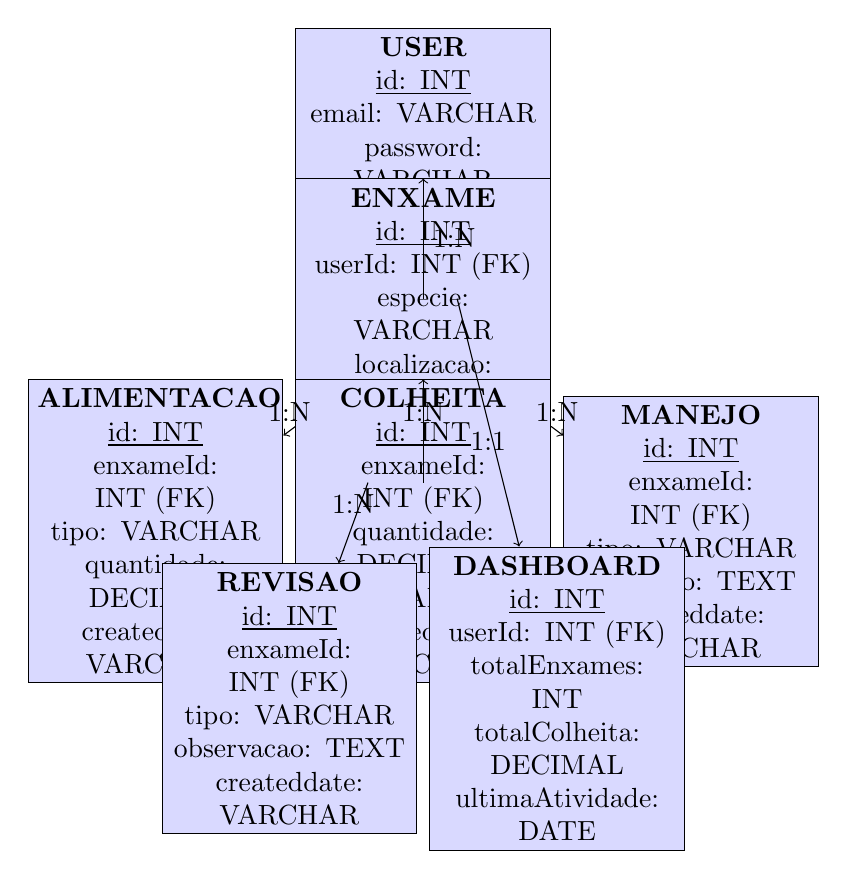
\begin{tikzpicture}[scale=0.85]
% Definição de estilos
\tikzset{
  table/.style={rectangle, draw, fill=blue!15, text width=3cm, text centered, minimum height=1.5cm},
  key/.style={rectangle, draw, fill=red!20, text width=2.8cm, text centered, minimum height=0.4cm},
  field/.style={rectangle, draw, fill=white, text width=2.8cm, text centered, minimum height=0.4cm}
}

% Tabela USER
\node[table] (user_table) at (0,8) {\textbf{USER}\\
\underline{id: INT}\\
email: VARCHAR\\
password: VARCHAR\\
planType: VARCHAR\\
status: VARCHAR};

% Tabela ENXAME
\node[table] (enxame_table) at (0,5.5) {\textbf{ENXAME}\\
\underline{id: INT}\\
userId: INT (FK)\\
especie: VARCHAR\\
localizacao: VARCHAR\\
forcaEnxame: VARCHAR};

% Tabela ALIMENTACAO
\node[table] (alimentacao_table) at (-4,2.5) {\textbf{ALIMENTACAO}\\
\underline{id: INT}\\
enxameId: INT (FK)\\
tipo: VARCHAR\\
quantidade: DECIMAL\\
createddate: VARCHAR};

% Tabela COLHEITA
\node[table] (colheita_table) at (0,2.5) {\textbf{COLHEITA}\\
\underline{id: INT}\\
enxameId: INT (FK)\\
quantidade: DECIMAL\\
tipo: VARCHAR\\
createddate: VARCHAR};

% Tabela MANEJO
\node[table] (manejo_table) at (4,2.5) {\textbf{MANEJO}\\
\underline{id: INT}\\
enxameId: INT (FK)\\
tipo: VARCHAR\\
descricao: TEXT\\
createddate: VARCHAR};

% Tabela REVISAO
\node[table] (revisao_table) at (-2,0) {\textbf{REVISAO}\\
\underline{id: INT}\\
enxameId: INT (FK)\\
tipo: VARCHAR\\
observacao: TEXT\\
createddate: VARCHAR};

% Tabela DASHBOARD
\node[table] (dashboard_table) at (2,0) {\textbf{DASHBOARD}\\
\underline{id: INT}\\
userId: INT (FK)\\
totalEnxames: INT\\
totalColheita: DECIMAL\\
ultimaAtividade: DATE};

% Relacionamentos
\draw[->] (user_table) -- node[right] {1:N} (enxame_table);
\draw[->] (enxame_table) -- node[above] {1:N} (alimentacao_table);
\draw[->] (enxame_table) -- node[above] {1:N} (colheita_table);
\draw[->] (enxame_table) -- node[above] {1:N} (manejo_table);
\draw[->] (enxame_table) -- node[above] {1:N} (revisao_table);
\draw[->] (user_table) -- node[below] {1:1} (dashboard_table);

\end{tikzpicture}
\label{fig:modelo-conceitual-banco}
\end{figura}